\documentclass[12pt]{article}
\usepackage{hyperref}
\usepackage[utf8]{inputenc}
\usepackage[T1]{fontenc}
\usepackage{graphicx}
\hypersetup{colorlinks=true,linkcolor=blue, linktocpage}
\begin{document}
\section*{Risengrynsgrøt, 03.01.2019}
\begin{itemize}
\item Oppskrift:
  \begin{itemize}
  \item Prøvde å sette grøten i ovnen, men en time etterpå hadde
    ingenting skjedd så gikk tilbake til f{\o}lgende
    \href{https://www.melk.no/Oppskrifter/Groeter/Tradisjonsgroet/Risengrynsgroet}{oppskrift}
    med 3~dl seterr{\o}mme.
  \end{itemize}
\item Kommentarer:
  \begin{itemize}
    \item Tok veldig lang tid (ca tre timer), vil nok kjøre på med
      høyere varme neste gang fra start og røre ofte. Satt seg ikke
      særlig fast i bunnen (overraskende).
  \end{itemize}
\item Konklusjon:
  \begin{itemize}
  \item Smakte helt ok, kanskje litt vassent, men vet ikke helt hvordan dette kan forbedres (lavere varme?). 
  \end{itemize}
\end{itemize}
\centering
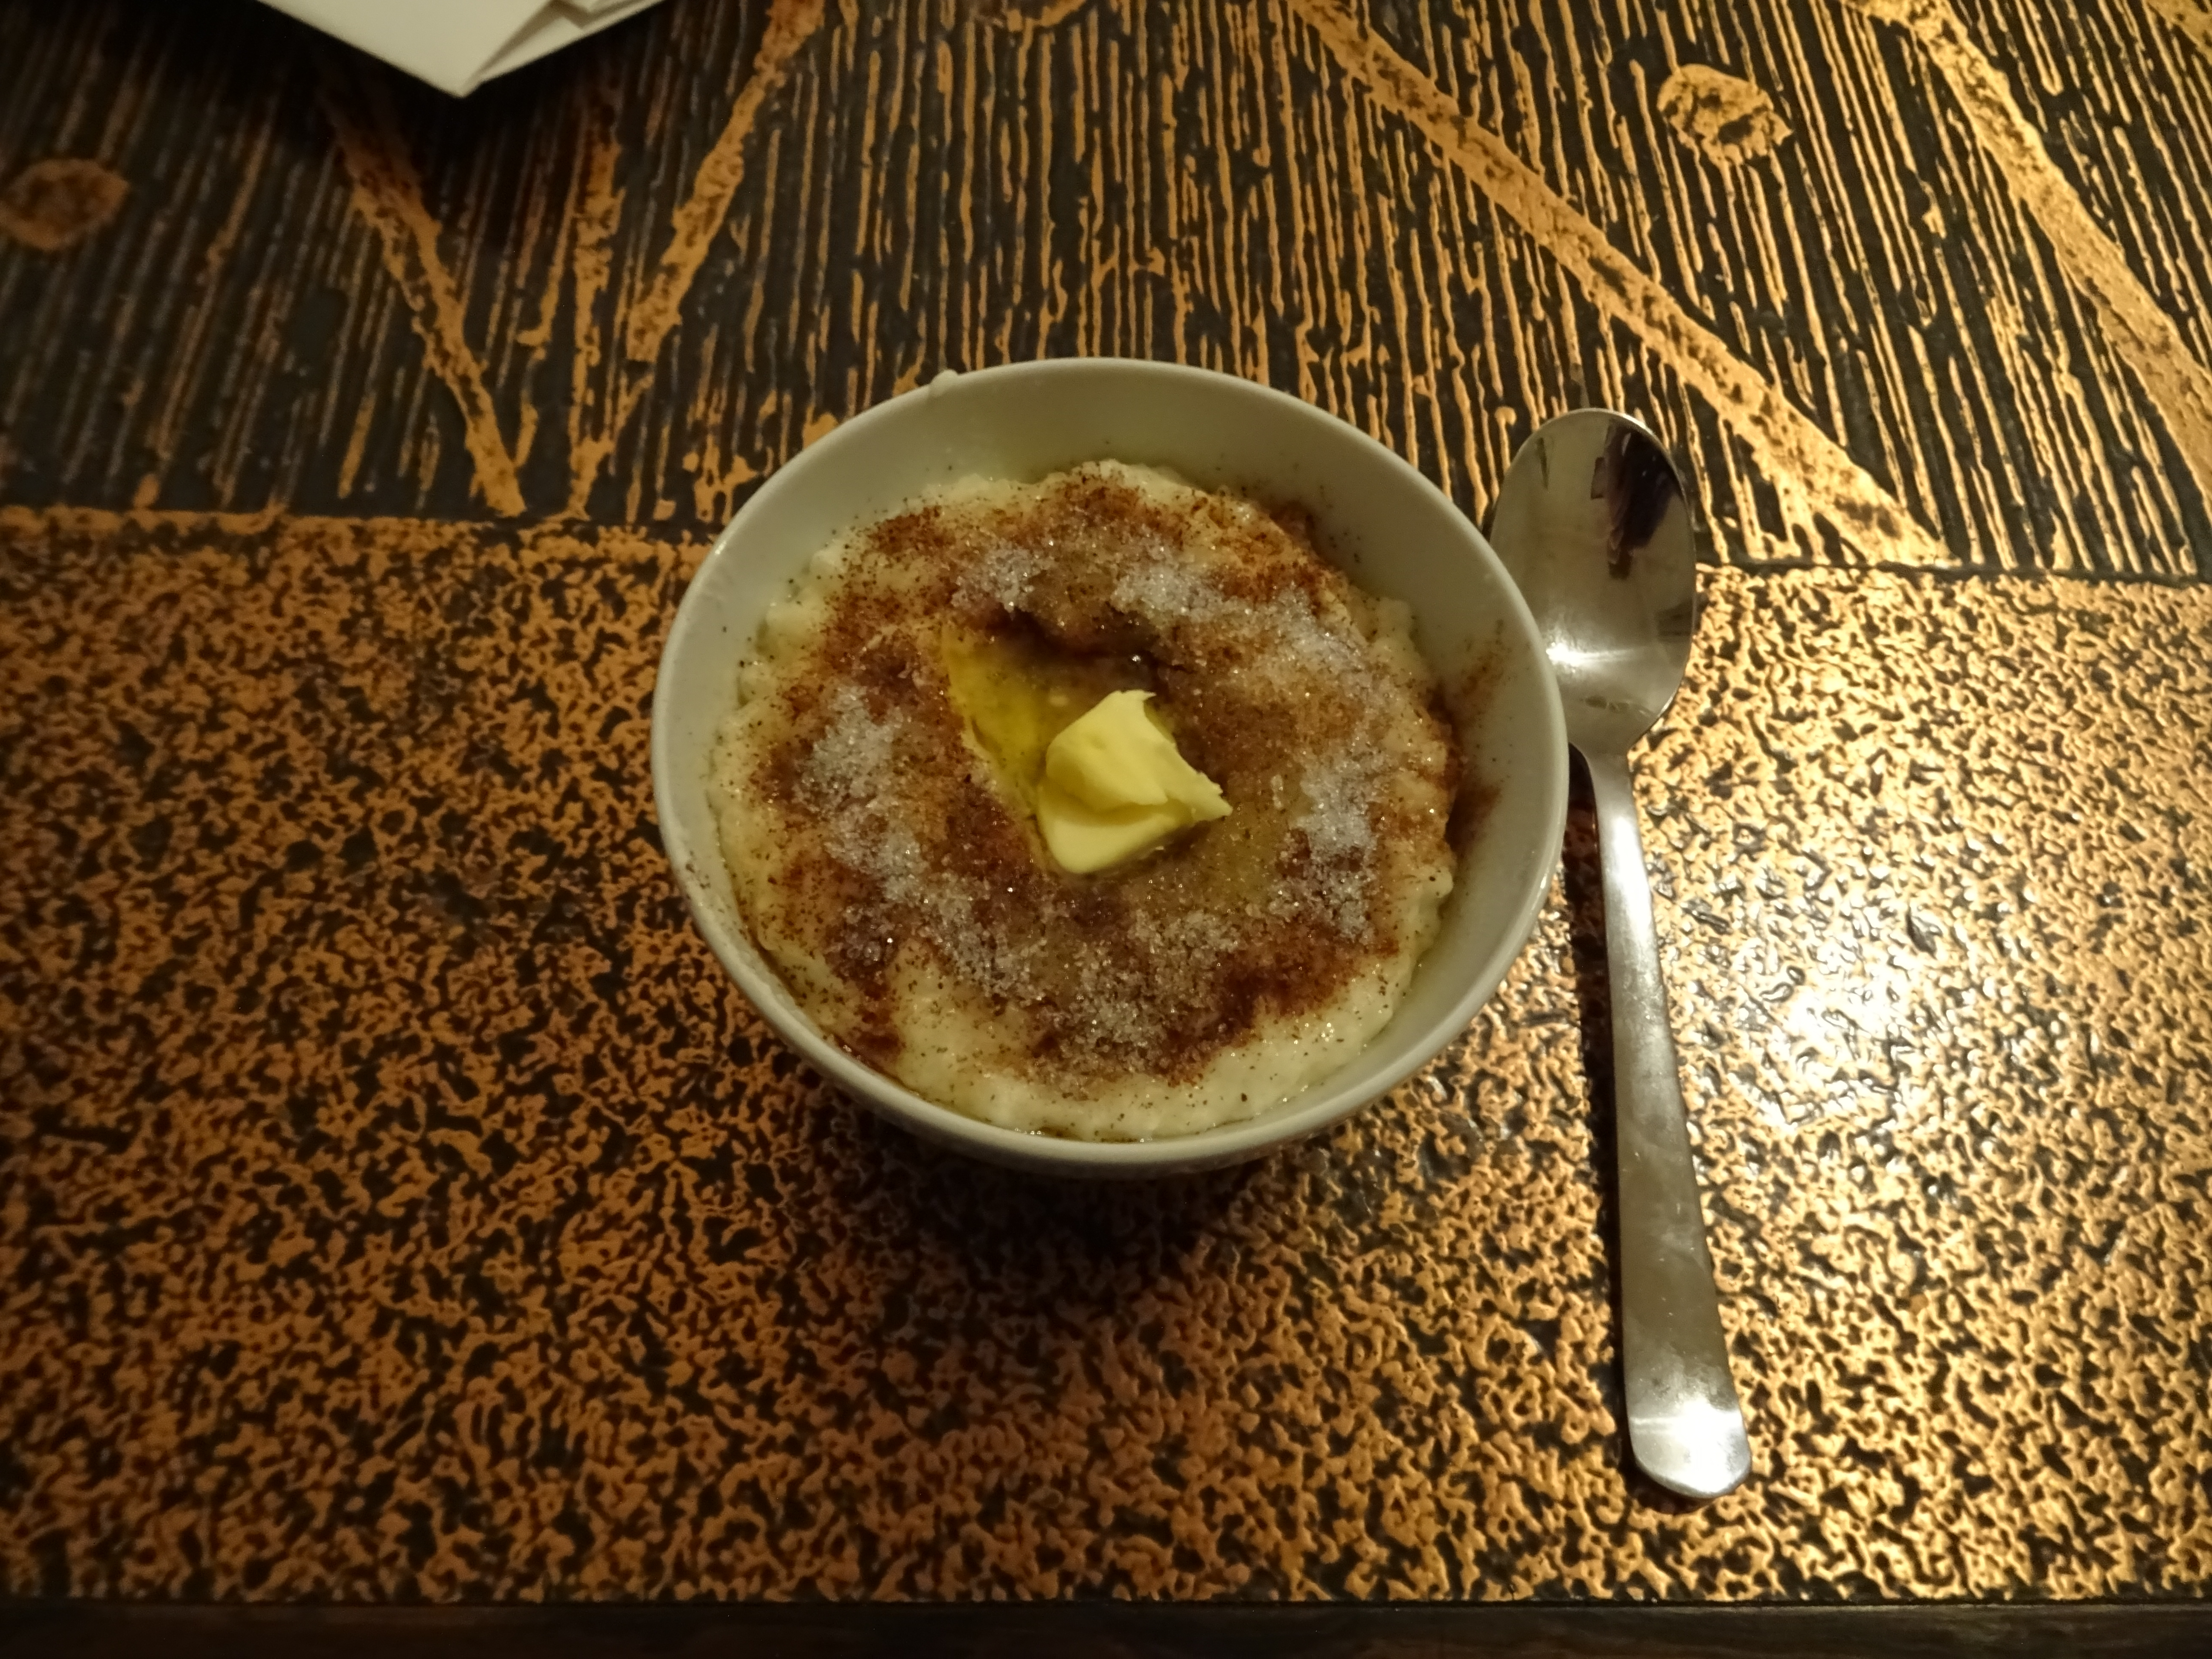
\includegraphics[width=0.33\textwidth]{03-01-2019.JPG}
\end{document}

